
\subsubsection{RQ1: Extraction Feasibility}

CV\_PR extraction succeeded for all 100 models tested (100\% completion rate).

\begin{table}[htbp]
\centering
\resizebox{\columnwidth}{!}{%
\begin{tabular}{ll}
\toprule
Metric & Value \\
\midrule
Models processed & 100 \\
Completion rate & 100\% \\
CV\_PR mean & 0.0116 \\
CV\_PR std & 0.0059 \\
CV\_PR min & 0.0014 \\
CV\_PR max & 0.0326 \\
\bottomrule
\end{tabular}
}
\end{table}

All CV\_PR values were finite and within expected range. The low absolute values (< 0.04) indicate that participation ratio estimates are consistent across random projections.

\subsubsection{RQ2: Correlation with Accuracy}

The hypothesis predicted r < -0.3. The observed correlation was positive.

\begin{table}[htbp]
\centering
\resizebox{\columnwidth}{!}{%
\begin{tabular}{ll}
\toprule
Statistic & Value \\
\midrule
Pearson r & +0.6065 \\
Pearson p & 9.24 $\times 10^{-11}$ \\
Spearman $\rho$ & +0.6368 \\
Spearman p & 5.26 $\times 10^{-12}$ \\
95\% CI & [0.506, 0.703] \\
n (matched) & 94 \\
\bottomrule
\end{tabular}
}
\end{table}

The hypothesis is falsified. CV\_PR shows a strong positive correlation with ImageNet accuracy. The 95\% confidence interval excludes all negative values and zero.

\begin{figure}[htbp]
\centering
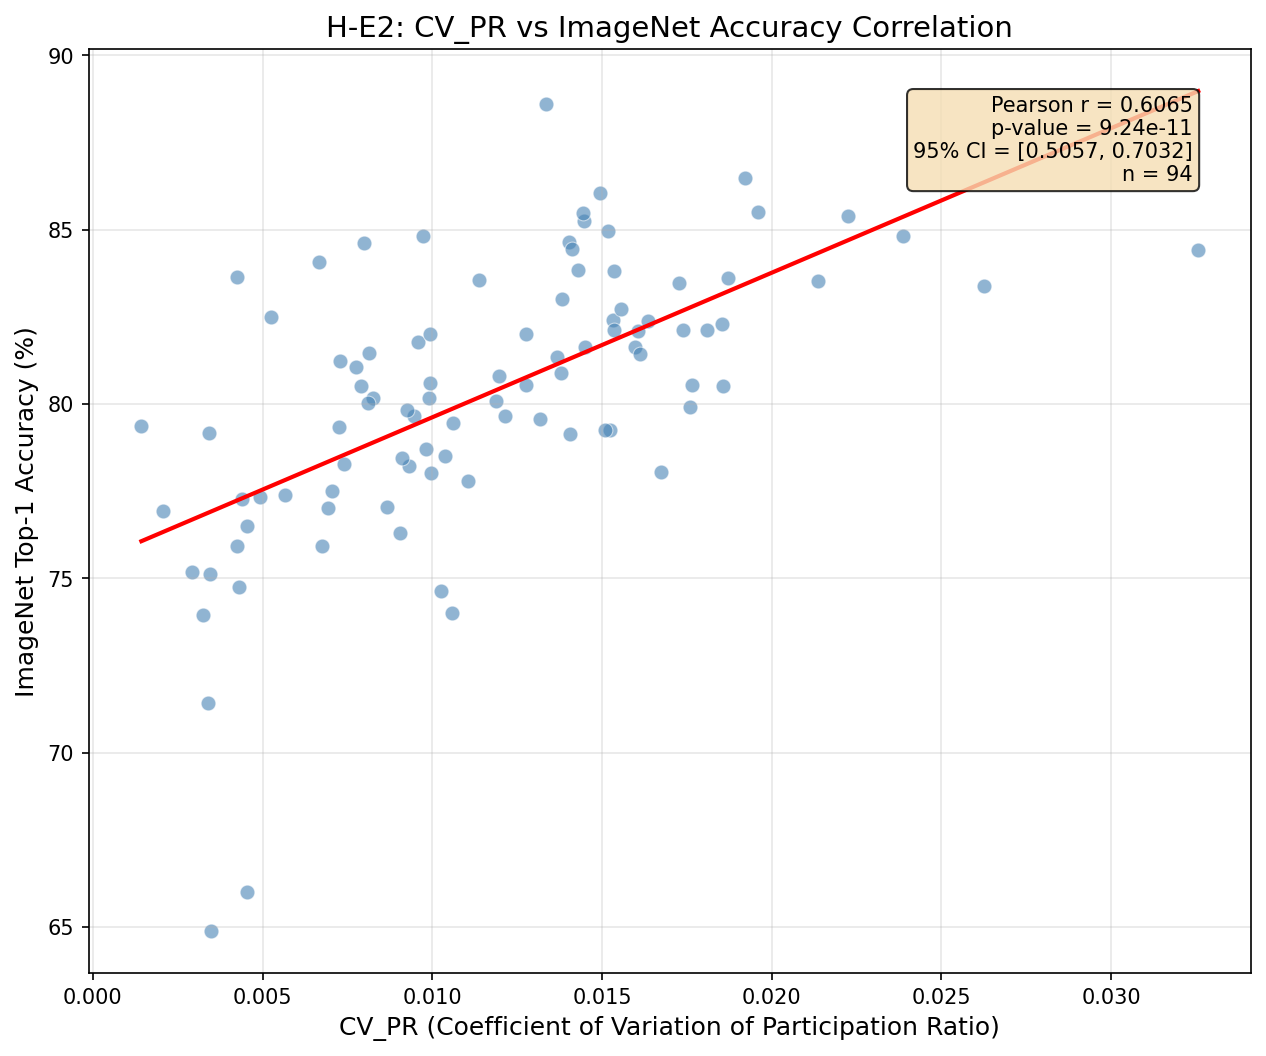
\includegraphics[width=\columnwidth]{figures/scatter_cv_pr_vs_accuracy.png}
\caption{CV\_PR vs Accuracy}
\label{fig:scatter_cv_pr_vs_accuracy}
\end{figure}

\textit{Figure 1: CV\_PR positively correlates with ImageNet top-1 accuracy (r = +0.61). Each point represents one pretrained model from timm. n = 94 matched models.}

\subsubsection{Data Quality}

\begin{table}[htbp]
\centering
\resizebox{\columnwidth}{!}{%
\begin{tabular}{lll}
\toprule
Variable & Mean & Std \\
\midrule
CV\_PR & 0.0116 & 0.0057 \\
Top-1 Accuracy & 80.3\% & 3.9\% \\
\bottomrule
\end{tabular}
}
\end{table}

Match rate between CV\_PR extraction and accuracy metadata: 94/100 (94\%). Six models lacked accuracy data in the timm results file.

\subsubsection{Outliers}

Two models with notably low CV\_PR and accuracy were identified:
\begin{itemize}
\item dla46\_c.in1k: CV\_PR = 0.0035, top1 = 64.88\%
\item dla46x\_c.in1k: CV\_PR = 0.0045, top1 = 66.01\%
\end{itemize}

These did not substantially affect the correlation.

\subsubsection{Summary}

\begin{table*}[htbp]
\centering
\resizebox{\dimexpr 2\columnwidth+\columnsep\relax}{!}{%
\begin{tabular}{lllll}
\toprule
Hypothesis & Gate & Criterion & Observed & Result \\
\midrule
H-E1 (Extraction) & MUST\_WORK & Completion $\geq$ 95\%, CV\_PR finite & 100\%, [0.0014, 0.0326] & PASS \\
H-E2 (Correlation) & MUST\_WORK & r < -0.3, p < 0.05 & r = +0.61, p < $10^{-10}$ & FAIL \\
\bottomrule
\end{tabular}
}
\end{table*}

The extraction methodology is validated. The negative correlation hypothesis is falsified with a complete directional reversal.
